%
% teil3.tex -- Beispiel-File für Teil 3
%
% (c) 2020 Prof Dr Andreas Müller, Hochschule Rapperswil
%
\section{Quaternionen}
\rhead{Quaternionen}

Wie die komplexen Zahlen eine Erweiterung der reellen Zahlen sind, sind die Quaternionen eine Erweiterung der komplexen Zahlen für den dreidimensionalen Raum. Sie haben, wie die komplexen Zahlen, eine dreh-streckende Eigenschaft.
Sie finden beispielsweise in der Computergraphik und in der Robotik Anwendung.
Die Quaternionen
\begin{align}
	q = w + xi + yj + zk \quad w,x,y,z \in \mathbb{R}\enspace q \in \mathbb{H}
\end{align}
können dabei eine Drehstreckung mit dieser Formel erreichen
\begin{align} \label{QuatRot}
	\begin{split} 
		&v'' = qvq^{-1};\quad q,v,q^{-1} \in \mathbb{H}\\
		&\operatorname{Re}(q) = \operatorname{Re}(q^{-1})\quad \operatorname{Im}(q) = -\operatorname{Im}(q^{-1})
	\end{split}
\end{align}
Auffallend ist hier schon die Ähnlichkeit zu dem Kapitel Rotation. Man könnte sich nun fragen wieso es drei imaginäre Einheiten $i,j,k$ gibt und nicht zwei, was doch näherliegender wäre. Der Grund liegt darin, weil es in der dritten Dimension drei Drehachsen gibt, anstatt nur eine. Wie im Kapitel Rotation beschrieben können wir auch hier die drei Drehungen durch Linearkombinationen von drei Bivektoren beschreiben. In der geometrischen Algebra ist es leicht herauszufinden wie viele Imaginärteile für jede weitere Dimension existieren. Dabei muss man nur die Anzahl der unabhängigen Bivektoren ermitteln. In der vierten Dimension würden es beispielsweise durch alle Vektorkombinationen von $\mathbf{e}_1, \mathbf{e}_2,\mathbf{e}_3, \mathbf{e}_4$ insgesamt 8 Bivektoren existieren (Nicht 16, da $\mathbf{e}_{ij} = -\mathbf{e}_{ji}$ nicht unabhängig voneinander sind).

Ohne die geometrische Algebra, haben wir jetzt aber leider ein kleines Problem. Für die Darstellung der Quaternionen bräuchten wir insgesamt vier Achsen. Drei für die imaginären Einheiten und eine für die reelle Einheit. Ein weiterer Nachteil in visueller Hinsicht entsteht beim Anwenden eines Quaternion auf einen Vektor. Sie befinden sich nicht im gleichen Raum und müssen zuerst ineinander umgewandelt werden, um damit zu rechnen, wie man bei $v \in \mathbb{H}$ in der Formel (\ref{QuatRot}) sieht.

\subsection{Geometrische Algebra}
Die geometrische Algebra besitzt die Fähigkeit beide Probleme zu lösen. Die Quaternionen können, wie schon im 2 dimensionalen Fall durch die gerade Grade $G_3^+(\mathbb{R}) \cong \mathbb{H}$ dargestellt werden. Da wir uns jetzt aber in $G_3(\mathbb{R})$ befinden haben wir drei Basisvektoren $\mathbf{e}_1, \mathbf{e}_2, \mathbf{e}_3$ und können somit drei Bivektoren bilden $\mathbf{e}_{12}, \mathbf{e}_{23}, \mathbf{e}_{31}$.
\begin{definition}
	Multivektoren mit Drehstreckenden Eigenschaften in $G_3(\mathbb{R})$ (gleichbedeutend zu Quaternionen)
	\begin{align}
		\mathbf{q} = w + x\mathbf{e}_{12} + y\mathbf{e_{23}} + z\mathbf{e_{31}}; \quad w,x,y,z \in \mathbb{R};\enspace \mathbf{q} \in \mathbb{G}_3^+
	\end{align}
\end{definition}

Die Probleme werden dadurch gelöst, da wir die Bivektoren im Raum nicht durch einzelne Achsen darstellen müssen, sondern sie als eine orientiere Fläche darstellen können. Anstatt die Vektoren in Quaternionen umzurechnen, können wir jetzt die Vektoren separat im gleichen Raum darstellen. 
\begin{figure}
	\centering
	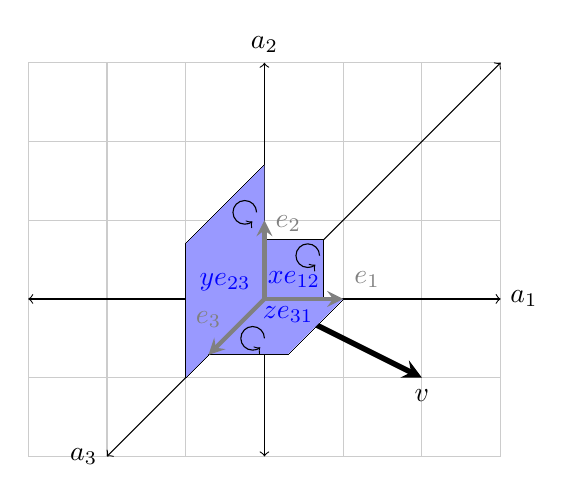
\begin{tikzpicture}
		% Koordinatensystem
		\draw[thin,gray!40] (-3,-2) grid (3,3);
		\draw[<->] (-3,0)--(3,0) node[right]{$a_1$};
		\draw[<->] (0,-2)--(0,3) node[above]{$a_2$};
		\draw[<->] (3,3)--(-2,-2) node[left]{$a_3$};
		
		% v Vektor
		\draw[line width=2pt,black,-stealth](0,0)--(2,-1) node[anchor=north]{$\boldsymbol{v}$};
		
		% q Quaternion
		\draw[line width=0,fill=blue!40] (0,0)--(0.75,0)--(0.75,0.75)--(0,0.75)
		node[xshift=0.375cm, yshift=-0.5cm, blue]{$x\boldsymbol{e_{12}}$};
		\draw[->] (0.7,0.55) arc (0:310:0.15);
		
		\draw[line width=0,fill=blue!40] (0,0)--(-1,-1)--(-1,0.71)--(0,1.71)
		node[xshift=-0.5cm, yshift=-1.5cm, blue]{$y\boldsymbol{e_{23}}$};
		\draw[->] (-0.1,1.1) arc (0:310:0.15);
		
		\draw[line width=0,fill=blue!40] (0,0)--(-0.71,-0.71)--(0.29,-0.71)--(1,0)
		node[xshift=-0.7cm, yshift=-0.2cm, blue]{$z\boldsymbol{e_{31}}$};
		\draw[->] (0,-0.5) arc (0:310:0.15);
		
		% Basisvektoren
		\draw[line width=1.5pt,gray,-stealth](0,0)--(1,0) node[anchor=south west]{$\boldsymbol{e_1}$};
		\draw[line width=1.5pt,gray,-stealth](0,0)--(0,1) node[anchor=north west, yshift=0.2cm]{$\boldsymbol{e_2}$};
		\draw[line width=1.5pt,gray,-stealth](0,0)--(-0.71,-0.71) node[anchor=south, yshift=0.2cm]{$\boldsymbol{e_3}$};
	\end{tikzpicture}
	\caption{Darstellung eines Quaternion $\mathbf{q}$ und eines Vektors $\mathbf{v}$ im selben Raum}
	\label{BildQuaternionen}
\end{figure}
Wie schon im 2 dimensionalen Fall beschreibt ein Bivektor, um wie viel der um 90 grad gedrehte orginale Vektor gestreckt wird. Dabei dreht jeder Bivektor den Vektor um eine andere Achse.
\\BILD?\\
In der Computergraphik und Robotik macht eine Drehstreckung aber nicht viel Sinn. Wieso sollte ein Objekt bei einer Drehung zusätzlich noch grösser werden? Darum verwendet man sogenannte Einheitsquaternionen, welche den Betrag $|q|=1$ haben. Sie rotieren die Objekte bzw. Vektoren lediglich.
\begin{definition}
	Einheitsquaternionen
	\begin{align}
		\mathbf{q} = \cos(\alpha) + sin(\alpha)(\tilde{x}\mathbf{e}_{12} + \tilde{y}\mathbf{e}_{23} + \tilde{z}\mathbf{e}_{31})
	\end{align}
\end{definition}
Dabei ist definiert, dass $\tilde{x}^2+\tilde{y}^2+\tilde{z}^2=1$. Somit beträgt der Betrag von $\mathbf{q}$ immer 1.
\begin{align}
	|\mathbf{q}| = \sqrt{cos(\alpha)^2 + sin(\alpha)^2(\tilde{x}^2+\tilde{y}^2+\tilde{z}^2) } = \sqrt{cos(\alpha)^2 + sin(\alpha)^2} = 1
\end{align}
Der Winkel $\alpha$ beschreibt dabei, wie im Bild (...) gezeigt den halben Winkel, um welchen der parallelen Anteil $\mathbf{v_{\perp}}$ des Vektors $\mathbf{v}$ zur kombinierten Bivektorebene $sin(\alpha)^2(\tilde{x}^2+\tilde{y}^2+\tilde{z}^2)$ gedreht wird.

Um einen Vektor zu drehen, verwendet man wieder die gleiche Formel, wie auch schon im zweidimensionalen Fall.
\begin{align} \label{QuatRotGA}
	\begin{split} 
		&\mathbf{v}'' = \mathbf{qvq}^{-1}\\
		&\operatorname{Re}(\mathbf{q}) = \operatorname{Re}(\mathbf{q}^{-1});\enspace \operatorname{Im}(\mathbf{q}) = -\operatorname{Im}(\mathbf{q}^-1)
	\end{split}
\end{align}
Es ist wichtig bei Quaternionen für eine reine Drehstreckung mit $q$ und $q^{-1}$ beidseitig zu multiplizieren, sonst werden die senkrechten Anteile zu den Bivektorebenen ebenfalls beeinflusst, wie man im Kapitel Rotation bei der Formel (\ref{RotAufPerpPar}) sehen kann.
\begin{beispiel}
	Eine Drehung eines Vektors $\mathbf{v}= 1\mathbf{e}_2$ um 90 Grad um die $\mathbf{e}_1$-Achse und danach 90 Grad um die $\mathbf{e}_2$-Achse. Dafür nehmen wir zuerst einen Einheitsquaternion welcher um die Orientierte Ebene $\mathbf{e}_{23}$ um 90 Grad dreht
	\begin{align}
		\mathbf{q}_{23} &= \cos(\pi/4) + sin(\pi/4)(1\mathbf{e}_{23}) =  e^{(\pi/4)\mathbf{e}_{23}} &= 0.71 + 0.71\mathbf{e}_{23}\\
		\mathbf{q}_{23}^{-1} &&= 0.71 - 0.71\mathbf{e}_{23}
	\end{align}
	und danach Einheitsquaternion welcher um die Orientierte Ebene $\mathbf{e}_{31}$ um 90 Grad dreht
	\begin{align}
		\mathbf{q}_{31} &= \cos(\pi/4) + sin(\pi/4)(1\mathbf{e}_{31}) =  e^{(\pi/4)\mathbf{e}_{31}} &= 0.71 + 0.71\mathbf{e}_{31}\\
		\mathbf{q}_{31}^{-1} &&= 0.71 - 0.71\mathbf{e}_{31}
	\end{align}
	Um die vollständige Rotation zu beschreiben können die  Einheitsquaternion multipliziert werden, wobei die Reihenfolge der Ausführung beachtet werden muss
	\begin{align} \label{FormelBeispielQuaternion}
		\mathbf{q} &= \mathbf{q}_{31}\mathbf{q}_{23} = (0.71 + 0.71\mathbf{e}_{31})(0.71 + 0.71\mathbf{e}_{23}) &= 0.5 + 0.5\mathbf{e}_{31} + 0.5 \mathbf{e}_{23} + 0.5 \mathbf{e}_{12}\\
		\mathbf{q}^{-1} &= \mathbf{q}_{23}^{-1}\mathbf{q}_{31}^{-1} = (0.71 - 0.71\mathbf{e}_{23})(0.71 - 0.71\mathbf{e}_{31}) &= 0.5 - 0.5\mathbf{e}_{31} - 0.5 \mathbf{e}_{23} - 0.5 \mathbf{e}_{12}
	\end{align}
	Wenn wir nun den Quaternion $\mathbf{q}$ auf den Vektor $\mathbf{v}$ anwenden
	\begin{align}
		\mathbf{v}'' = \mathbf{qvq}^{-1} &= (0.5 + 0.5\mathbf{e}_{31} + 0.5 \mathbf{e}_{23} + 0.5 \mathbf{e}_{12})(1\mathbf{e}_2)(0.5 - 0.5\mathbf{e}_{31} - 0.5 \mathbf{e}_{23} - 0.5 \mathbf{e}_{12})\\ 
		&= (0.5\mathbf{e}_2 + 0.5 \mathbf{e}_{123} - 0.5 \mathbf{e}_3 + 0.5 \mathbf{e}_1)(0.5 - 0.5\mathbf{e}_{31} - 0.5 \mathbf{e}_{23} - 0.5 \mathbf{e}_{12})\\
		&= (0.25 + 0.25 + 0.25 + 0.25)\mathbf{e}_1 + (0.25 + 0.25 - 0.25 - 0.25)\mathbf{e}_2 +\\ &(-0.25 + 0.25 - 0.25 + 0.25)\mathbf{e}_3 + (0.25 - 0.25 - 0.25 + 0.25)\mathbf{e}_{123}\\
		&= 1e_1 
	\end{align}
	Anders betrachtet könnte man von der Formel \eqref{FormelBeispielQuaternion} sehen, dass der Drehwinkel
	\begin{align}
		\alpha = \arccos(w) = \arccos(0.5) = 60°
	\end{align}
	und die Ebene der kombinierten Bivektoren wie in Abbildung \ref{BildQuaternionBeispiel2} aussieht.
	Somit kann man sich ebenfalls Vorstellen, wie der parallele Anteil zur Ebene insgesamt um 120° rotiert wird während der senkrechte Anteil unverändert bleibt
\end{beispiel}

\begin{figure}
	\centering
	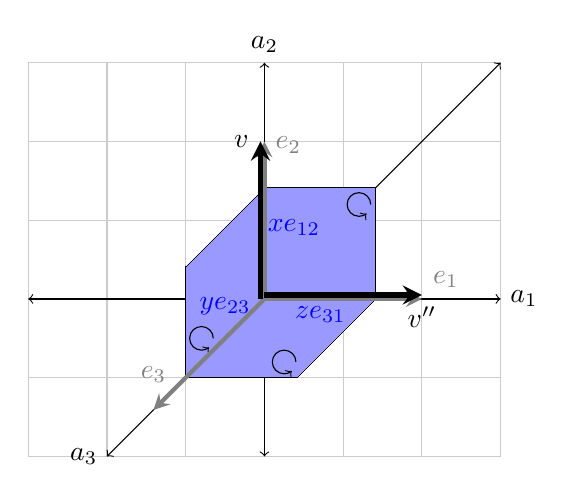
\begin{tikzpicture}
		% Koordinatensystem
		\draw[thin,gray!40] (-3,-2) grid (3,3);
		\draw[<->] (-3,0)--(3,0) node[right]{$a_1$};
		\draw[<->] (0,-2)--(0,3) node[above]{$a_2$};
		\draw[<->] (3,3)--(-2,-2) node[left]{$a_3$};
		
		% q Quaternion
		\draw[line width=0,fill=blue!40] (0,0)--(1.41,0)--(1.41,1.41)--(0,1.41)
		node[xshift=0.375cm, yshift=-0.5cm, blue]{$x\boldsymbol{e_{12}}$};
		\draw[->] (1.35, 1.2) arc (0:310:0.15);
		
		\draw[line width=0,fill=blue!40] (0,0)--(-1,-1)--(-1,0.41)--(0,1.41)
		node[xshift=-0.5cm, yshift=-1.5cm, blue]{$y\boldsymbol{e_{23}}$};
		\draw[->] (-0.65,-0.5) arc (0:310:0.15);
		
		\draw[line width=0,fill=blue!40] (0,0)--(-1,-1)--(0.41,-1)--(1.41,0)
		node[xshift=-0.7cm, yshift=-0.2cm, blue]{$z\boldsymbol{e_{31}}$};
		\draw[->] (0.4,-0.8) arc (0:310:0.15);
		
		% Basisvektoren
		\draw[line width=1.5pt,gray,-stealth](0,0)--(2,0) node[anchor=south west]{$\boldsymbol{e_1}$};
		\draw[line width=1.5pt,gray,-stealth](0,0)--(0,2) node[anchor=north west, yshift=0.2cm]{$\boldsymbol{e_2}$};
		\draw[line width=1.5pt,gray,-stealth](0,0)--(-1.41,-1.41) node[anchor=south, yshift=0.2cm]{$\boldsymbol{e_3}$};
		
		% v Vektor
		\draw[line width=2pt,black,-stealth](-0.05,0)--(-0.05,2) node[anchor=east]{$\boldsymbol{v}$};
		% v'' Vektor
		\draw[line width=2pt,black,-stealth](0,0.05)--(2,0.05) node[anchor=north]{$\boldsymbol{v}''$};
	\end{tikzpicture}
	\caption{Beispiel für Drehung um 90 Grad je um die $\mathbf{e}_1$- und $\mathbf{e}_2$-Achse.}
	\label{BildQuaternionBeispiel}
\end{figure}

\begin{figure}
	\centering
	\begin{tikzpicture}
		% q Quaternion
		\draw[line width=0,fill=blue!40] (-0.75,-1)--(1.5,-0.5)--(0.55,1.35)--(-1.5,1)
		node[xshift=0.375cm, yshift=-0.5cm, blue]{$\boldsymbol{q}$};
		\draw[->] (-0.7, 0.5) arc (310:0:0.15);
		
		% Koordinatensystem
		\draw[thin,gray!40] (-3,-2) grid (3,3);
		\draw[<->] (-3,0)--(3,0) node[right]{$a_1$};
		\draw[<->] (0,-2)--(0,3) node[above]{$a_2$};
		\draw[<->] (3,3)--(-2,-2) node[left]{$a_3$};
		
		% Basisvektoren
		\draw[line width=1.5pt,gray,-stealth](0,0)--(2,0) node[anchor=south west]{$\boldsymbol{e_1}$};
		\draw[line width=1.5pt,gray,-stealth](0,0)--(0,2) node[anchor=north west, yshift=0.2cm]{$\boldsymbol{e_2}$};
		\draw[line width=1.5pt,gray,-stealth](0,0)--(-1.41,-1.41) node[anchor=south, yshift=0.2cm]{$\boldsymbol{e_3}$};
		
		% v Vektor
		\draw[line width=2pt,black,-stealth](-0.05,0)--(-0.05,2) node[anchor=east]{$\boldsymbol{v}$};
		% vpar Vektor
		\draw[line width=2pt,red,-stealth](0,0)--(-0.33,1.25) node[anchor=east]{$\boldsymbol{v_{\parallel}}$};
		% vperp Vektor
		\draw[line width=2pt,green,-stealth](-0.33,1.25)--(0,2) node[anchor=east, xshift = -0.05, yshift = -0.3cm]{$\boldsymbol{v_{\perp}}$};
		% v'' Vektor
		\draw[line width=2pt,black,-stealth](0,0.05)--(2,0.05) node[anchor=north, xshift = 0.25cm]{$\boldsymbol{v}''$};
		% vpar'' Vektor
		\draw[line width=2pt,red,-stealth](0,0)--(1.66,-0.75) node[anchor=east, yshift = -0.2cm, xshift = -0.1cm]{$\boldsymbol{v_{\parallel}''}$};
		% vperp'' Vektor
		\draw[line width=2pt,green,-stealth](1.66,-0.75)--(2,0) node[anchor=east, xshift = 0.5cm, yshift = -0.65cm]{$\boldsymbol{v_{\perp}''}$};
		
		\coordinate (A) at (0,0);
		\coordinate (B) at (-0.33,1.25);
		\coordinate (C) at (1.66,-0.75);
		\tikzset{anglestyle/.style={angle eccentricity=2, draw,  thick, angle radius=0.75cm, purple}}
		\draw pic ["120° $=2\alpha$", anglestyle] {angle = C--A--B};
	\end{tikzpicture}
	\caption{Beim Beispiel wird der parallele Anteil um 120° gedreht während der senkrechte Anteil zur kombinierten Ebene (Bivektoraddition) gleich bleibt}
	\label{BildQuaternionBeispiel2}
\end{figure}

\subsection{Interpolation}
In der Computergrafik wird Interpolation verwendet, um eine flüssige Drehbewegung zu erreichen. Dabei wird die gewünschte Drehbewegungen des Objektes in kleinere aufgeteilt. Man kann dabei mit zwei verschiedenen Systemen arbeiten. 
\begin{itemize}
	\item Mit den Eulerschen Winkeln, welche für die Meisten zwar intuitiver sind, aber dafür Nachteile haben, worauf ich in diesem Abschnitt eingehen werde. Dabei kann eine ganze Drehbewegung $\mathbf{v}'' = R\mathbf{v}$ durch die Drehmatrix $R$ dargestellt werden. 
	\begin{align}
		\begin{split}
			&R = R_z(\gamma) R_y(\beta) R_x(\alpha)\\
			&R = 
			\begin{pmatrix} 
				\cos(\gamma) & -\sin(\gamma) & 0\\ \sin(\gamma) & \cos(\gamma) & 0 \\ 0 & 0 & 1 
			\end{pmatrix}
			\begin{pmatrix}
				\cos(\beta) &  0 & \sin(\beta)\\ 0 & 1 & 0 \\ -\sin(\beta) & 0 & \cos(\beta)
			\end{pmatrix}
			\begin{pmatrix} 
				1 & 0 & 0 \\ 0 & \cos(\alpha) & -\sin(\alpha)\\ 0 & \sin(\alpha) & \cos(\alpha)
			\end{pmatrix}
		\end{split}
	\end{align}
	Wichtig dabei zu sehen ist, dass die Drehbewegungen durch die einzelnen Matrizen nacheinander ausgeführt werden. Das bedeutet, wenn man die Reihenfolge vertauscht, bekommt man eine völlig andere Drehung. Man kann die Auswirkungen der Reihenfolge gut bei einem Gimbal (REF zu BILD) sehen. Die Matrix ganz links ist die, welche als letztes Angewendet wird. Somit bildet sie die Drehung des äusseren Rings, welche auch die zwei inneren Ringe und das Objekt mitdreht. Die Matrix ganz rechts hingegen bildet nur die Drehung des inneren Rings, welche nur das Objekt selber dreht. Man kann dabei erkennen, dass vorgehen dabei sehr intuitiv ist, aber es kompliziert sein kann eine gewünschte Drehbewegung auszuführen, da sich beim Drehen der äusseren Achse, sich auch die Inneren drehen. Das bedeutet, wenn man sich eine Drehbewegung um die anfängliche x Achse mit $R_x(\alpha_2)$ wünscht, und vorher eine beliebige Drehung $R = R_z(\gamma_1) R_y(\beta_1) R_x(\alpha_1)$ ausgeführt hat, bekommt man nicht das richtige Ergebnis, da die anfängliche x-Achse durch die Drehmatrizen $R_z(\gamma_1)$ und $R_y(\beta_1)$ zu einer neuen, lokalen x-Achse wurde. 
	\item Andererseits mit den Quaternionen, welche die besondere Eigenschaft haben, dass eine Drehung immer um die globale Achsen ausgeführt wird, egal in welcher Rotationsposition sich das Objekt befindet.
\end{itemize}
Für Spielentwickler ist es darum meist sinnvoller Quaternionen für Drehbewegungen anzuwenden, als sich mit komplizierten Berechnungen mit Eulerschen Winkeln herumzuschlagen.
\subsection{Gimbal-Lock}
Ein weiterer Nachteil der Eulerschen Winkel ist das Gimbal-Lock. Es entsteht dann, wenn der äussere Ring Deckungsgleich über denn Inneren gedreht wird. Dabei verliert das Gimbal eine Drehrichtung, da der äussere und Innere Ring nun die gleiche Drehrichtung besitzen. Dies kann beispielsweise Probleme bei Spielen bei der Berechnung der Interpolation führen. Man hat das bei älteren Spielen dann gesehen, wenn plötzlich Gliedmassen bei den Spielermodellen in unnatürlichen Richtungen gesprungen sind.
\subsection{Fazit}
andere Darstellungsweise. Besser für Verständnis => komplexe Zahlen erscheinen ähnlicher zu Quaternionen? Eine Sprache für alle Geometrische Probleme